\documentclass[10pt,final,a4paper,oneside,onecolumn]{article}

%%==========================================================================
%% Packages
%%==========================================================================
\usepackage[a4paper,left=3.5cm,right=3.5cm,top=3cm,bottom=3cm]{geometry} %% change page layout; remove for IEEE paper format
\usepackage[T1]{fontenc}                        %% output font encoding for international characters (e.g., accented)
\usepackage[cmex10]{amsmath}                    %% math typesetting; consider using the [cmex10] option
\usepackage{amssymb}                            %% special (symbol) fonts for math typesetting
\usepackage{amsthm}                             %% theorem styles
\usepackage{dsfont}                             %% double stroke roman fonts: the real numbers R: $\mathds{R}$
\usepackage{mathrsfs}                           %% formal script fonts: the Laplace transform L: $\mathscr{L}$
\usepackage[pdftex]{graphicx}                   %% graphics control; use dvips for TeXify; use pdftex for PDFTeXify
\usepackage{array}                              %% array functionality (array, tabular)
\usepackage{upgreek}                            %% upright Greek letters; add the prefix 'up', e.g. \upphi
\usepackage[noadjust]{cite}                     %% citations; noadjust removes leading spaces
%\usepackage[round]{natbib}                     %% Author-year citations (remove package cite)
\usepackage{stfloats}                           %% improved handling of floats
\usepackage{multirow}                           %% cells spanning multiple rows in tables
%\usepackage{subfigure}                         %% subfigures and corresponding captions (for use with IEEEconf.cls)
\usepackage{subfig}                             %% subfigures (IEEEtran.cls: set caption=false)
\usepackage{fancyhdr}                           %% page headers and footers
\usepackage[official,left]{eurosym}             %% the euro symbol; command: \euro
\usepackage{appendix}                           %% appendix layout
\usepackage{xspace}                             %% add space after macro depending on context
\usepackage{verbatim}                           %% provides the comment environment
\usepackage[dutch,USenglish]{babel}             %% language support
\usepackage{wrapfig}                            %% wrapping text around figures
\usepackage{longtable}                          %% tables spanning multiple pages
\usepackage{pgfplots}                           %% support for TikZ figures (Matlab)
\pgfplotsset{compat=1.9}
\usepackage[breaklinks=true,hidelinks,          %% implement hyperlinks (dvips yields minor problems with breaklinks;
bookmarksnumbered=true]{hyperref}   %% IEEEtran: set bookmarks=false)
%\usepackage[hyphenbreaks]{breakurl}            %% allow line breaks in URLs (don't use with PDFTeX)
\usepackage[final]{pdfpages}                    %% Include other pdfs

%%==========================================================================
%% Define header/title stuff
%%==========================================================================
\newcommand{\progressreportnumber}{3}
\renewcommand{\author}{Erwin de Gelder}
\renewcommand{\date}{18 December 2017}
\renewcommand{\title}{Performance assessment of automated vehicles using real-life driving scenarios}

%%==========================================================================
%% Fancy headers and footers
%%==========================================================================
\pagestyle{fancy}                                       %% set page style
\fancyhf{}                                              %% clear all header & footer fields
\fancyhead[L]{Progress report \progressreportnumber}    %% define headers (LE: left field/even pages, etc.)
\fancyhead[R]{\author, \date}                           %% similar
\fancyfoot[C]{\thepage}                                 %% define footer

\begin{document}
	
\begin{center}
	\begin{tabular}{c}
		\title \\ \\
		\textbf{\huge Progress report \progressreportnumber} \\ \\
		\author \\ 
		\date
	\end{tabular}
\end{center}

\section{Previous meeting minutes}

\begin{itemize}
	\item TNO is processing the contract between TU Delft and TNO. To be continued.
	\item Main purpose of the meeting was to discuss the definitions of scenario and event.
	\item Regarding the definition of scenario: the fact that it is possible to describe the scenario (which is quantitative) can be described in qualitative manners should not be part of the definition. It should be a result of the definition.
	\item For the definition of event, it was stated that the time interval between two consecutive events could be semantically described. This should not be part of the definition, but a result from the definition.
	\item There was some debate about the word `model'. It is stated that $x=f_\theta(t)$ ($x$ being the state, $\theta$ begin a parameter vector) is a model, though is would actually be a solution of, e.g., the `model' $\dot{x}=f_\theta(x, t)$.
	\item We agreed that it would be good to write a conference paper regarding the ontology of real-life scenario for automotive application. Paper will be submitted to IV2018, deadline 15th of January, 2018.
\end{itemize}

\section{Summary of work}

\begin{itemize}
	\item Regarding my PhD, I focussed on writing the paper. 
\end{itemize}

\section{Future plans}

\begin{itemize}
	\item Short term: submit paper for IV2018.
	\item Long term: finally, it looks like as if I will have access to real-life driving data soon. I have two activities in mind that I want to carry out as soon as I have access to the data:
	\begin{itemize}
		\item Detect a very simple and frequent scenario (e.g., braking of the ego vehicle). I want to see whether the variety of this simple and frequent scenario can be useful for a case study on \emph{completeness}.
		\item There should be annotations of ``challenging scenarios'', so it should be possible to have multiple `challenging scenarios'' of a specific scenario class. For example, scenarios in which a pedestrian crosses the road while the ego vehicle is approaching. I want to see if it is possible to generate the same type of scenarios using the parametrization of the recorded scenarios.
	\end{itemize}
\end{itemize}

\section{Questions}

\begin{itemize}
	\item Attached is the draft paper. I welcome any feedback, but particularly on the following I would appreciate feedback:
	\begin{itemize}
		\item The overall structure of the paper.
		\item Section~I (the introduction).
		\item Section~II-A (the context of this paper).
		\item Section~II-B (definition of scenario).
		\item Section~II-D (definition of event).
	\end{itemize}
	Note that I want to add a figure for Section~II-B which should summarize the details written in this section. I still have to finish this. If this is finished before the meeting, I will share it with you.
	\item What would be an appropriate name for the time interval between two events. For example, the moment a vehicle starts braking is an event and the moment the vehicle stops braking is also an event. As a result, within the time interval between these two events, the particular vehicle is braking. In this particular case, we can refer to this time interval with the term `braking', but I wonder if there is a more general term for this. 
\end{itemize}

%\bibliographystyle{ieeetr}
%\bibliography{../../bib}

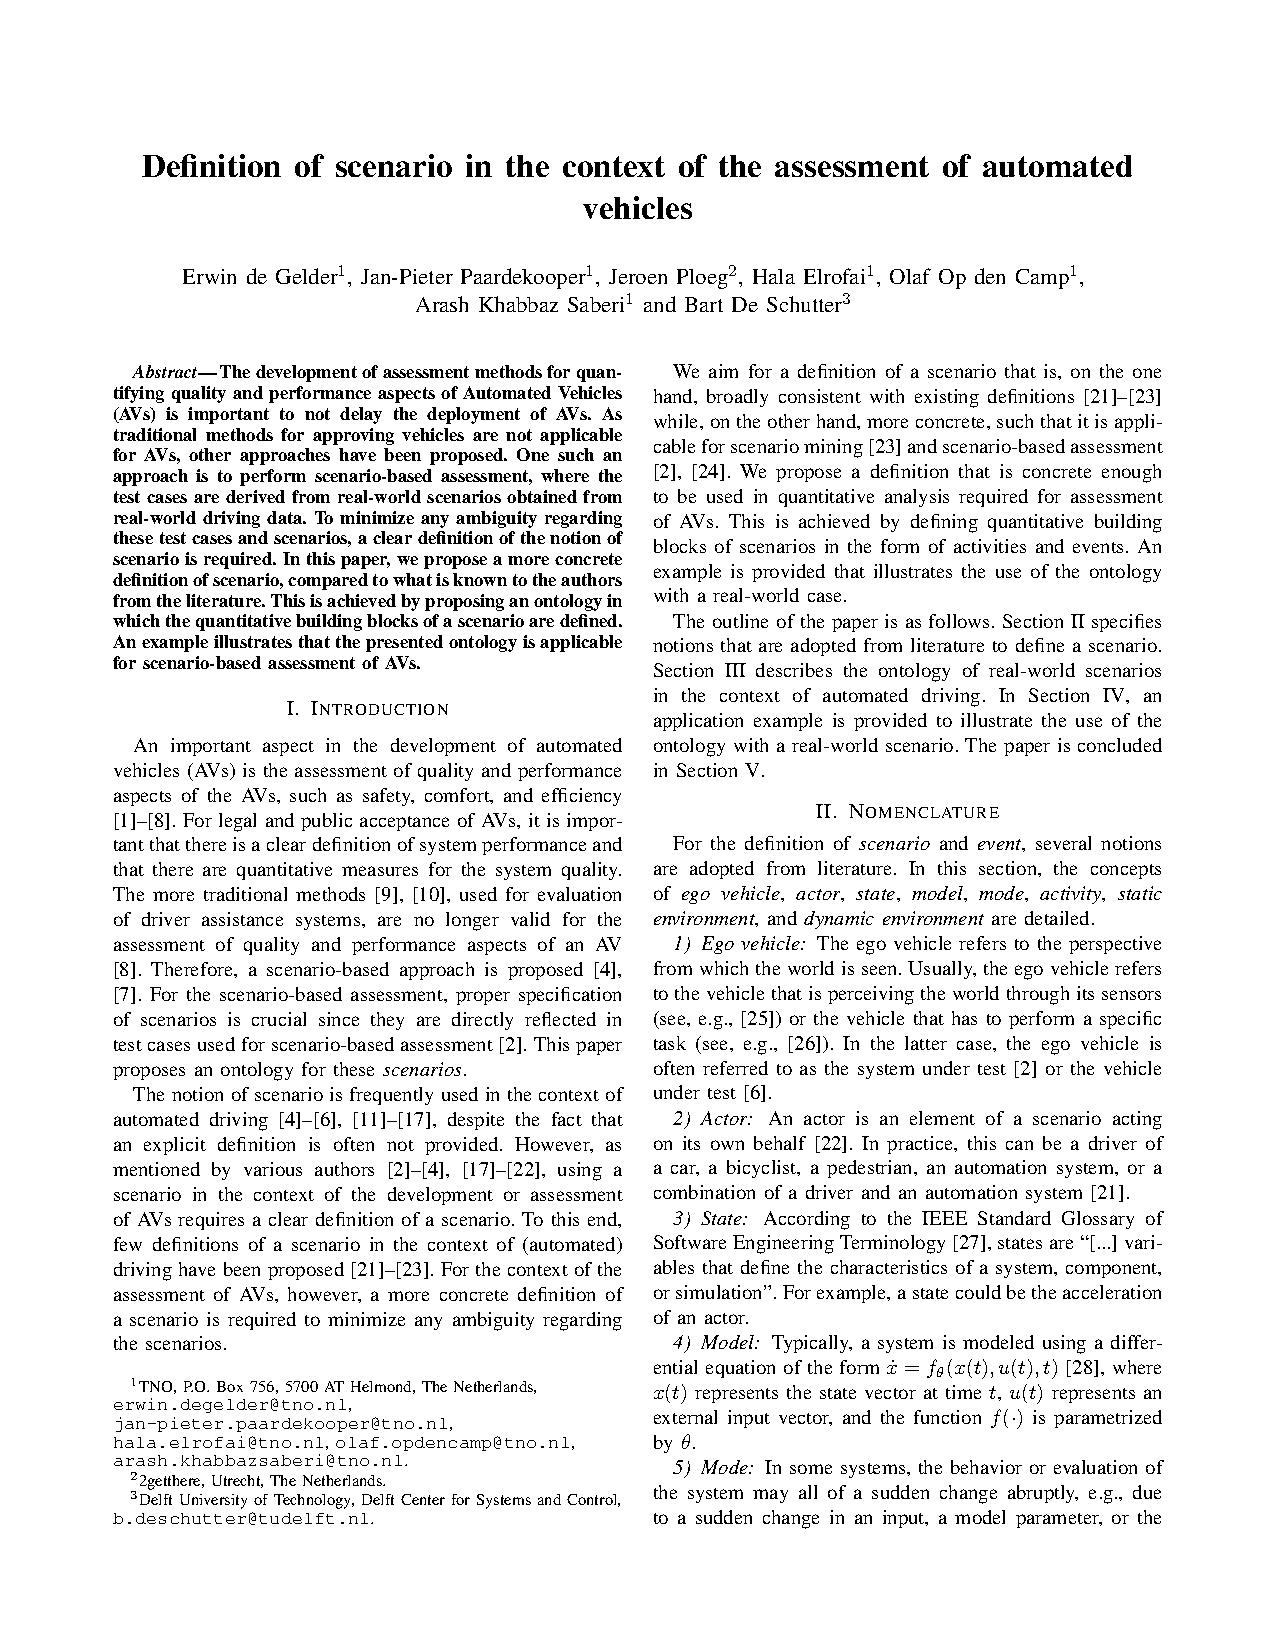
\includepdf[pages=-,pagecommand={},width=\paperwidth]{../../"20171111 IV2018 Ontology"/ontology.pdf}

\end{document}